\documentclass[Main.tex]{subfiles}
\begin{document}
	\section{An toàn trong phòng thực hành}
	\subsection{Lý thuyết}
	\begin{kienthuccannho}
		\subsubsection{Một số kí hiệu cảnh báo trong phòng thực hành}
		\begin{center}
			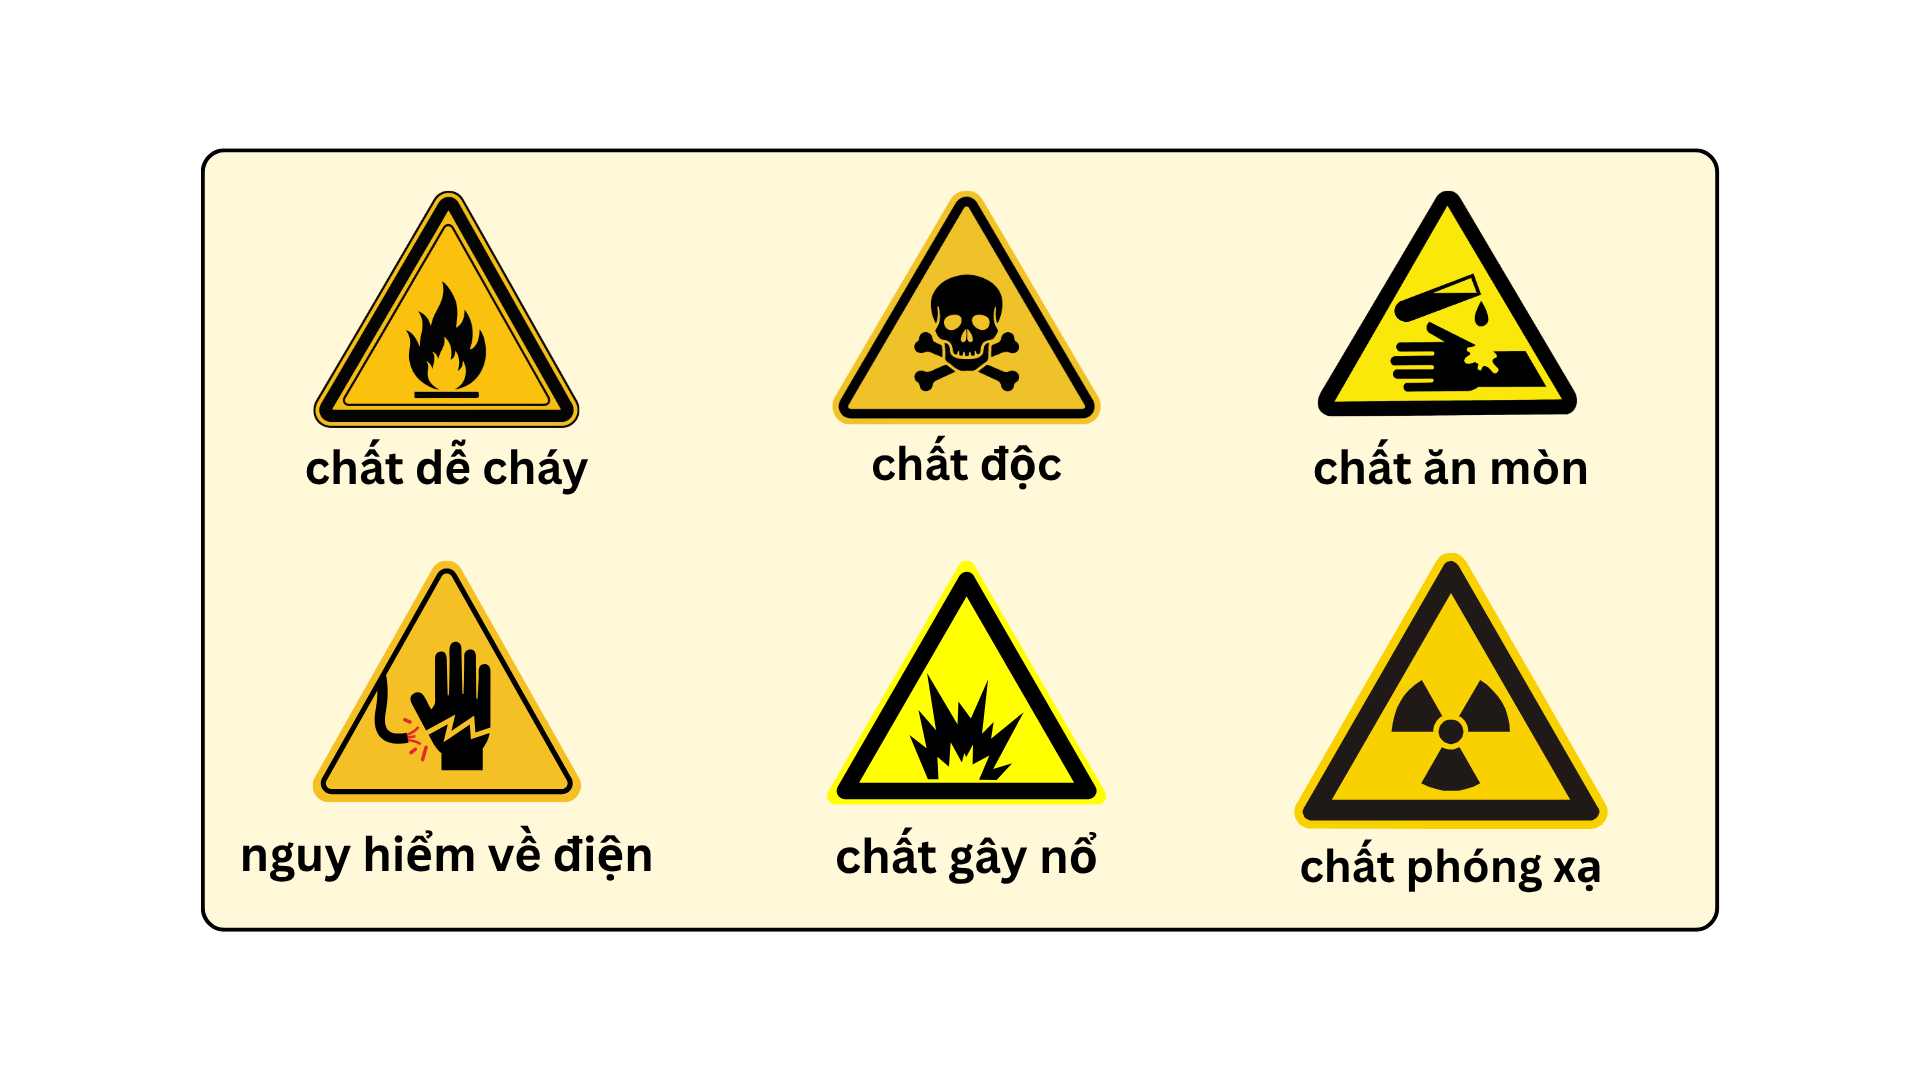
\includegraphics[width=0.98\linewidth,trim=3cm 3.8cm 3cm 3.8cm,clip]{Images/DE_CUONG_HOA_6_HKI/bien_bao.png}
			\captionof{figure}{\textbf{\textit{Một số kí hiệu cảnh báo phòng thí nghiệm}} }
		\end{center}
		Các kí hiệu cảnh báo trong phòng thực hành giúp nhận biết nhanh các nguy cơ như chất dễ cháy, chất độc, chất ăn mòn, nguy hiểm về điện, chất gây nổ, chất phóng xạ, $\ldots$
		\subsubsection{An toàn trong phòng thực hành}
		\begin{center}
		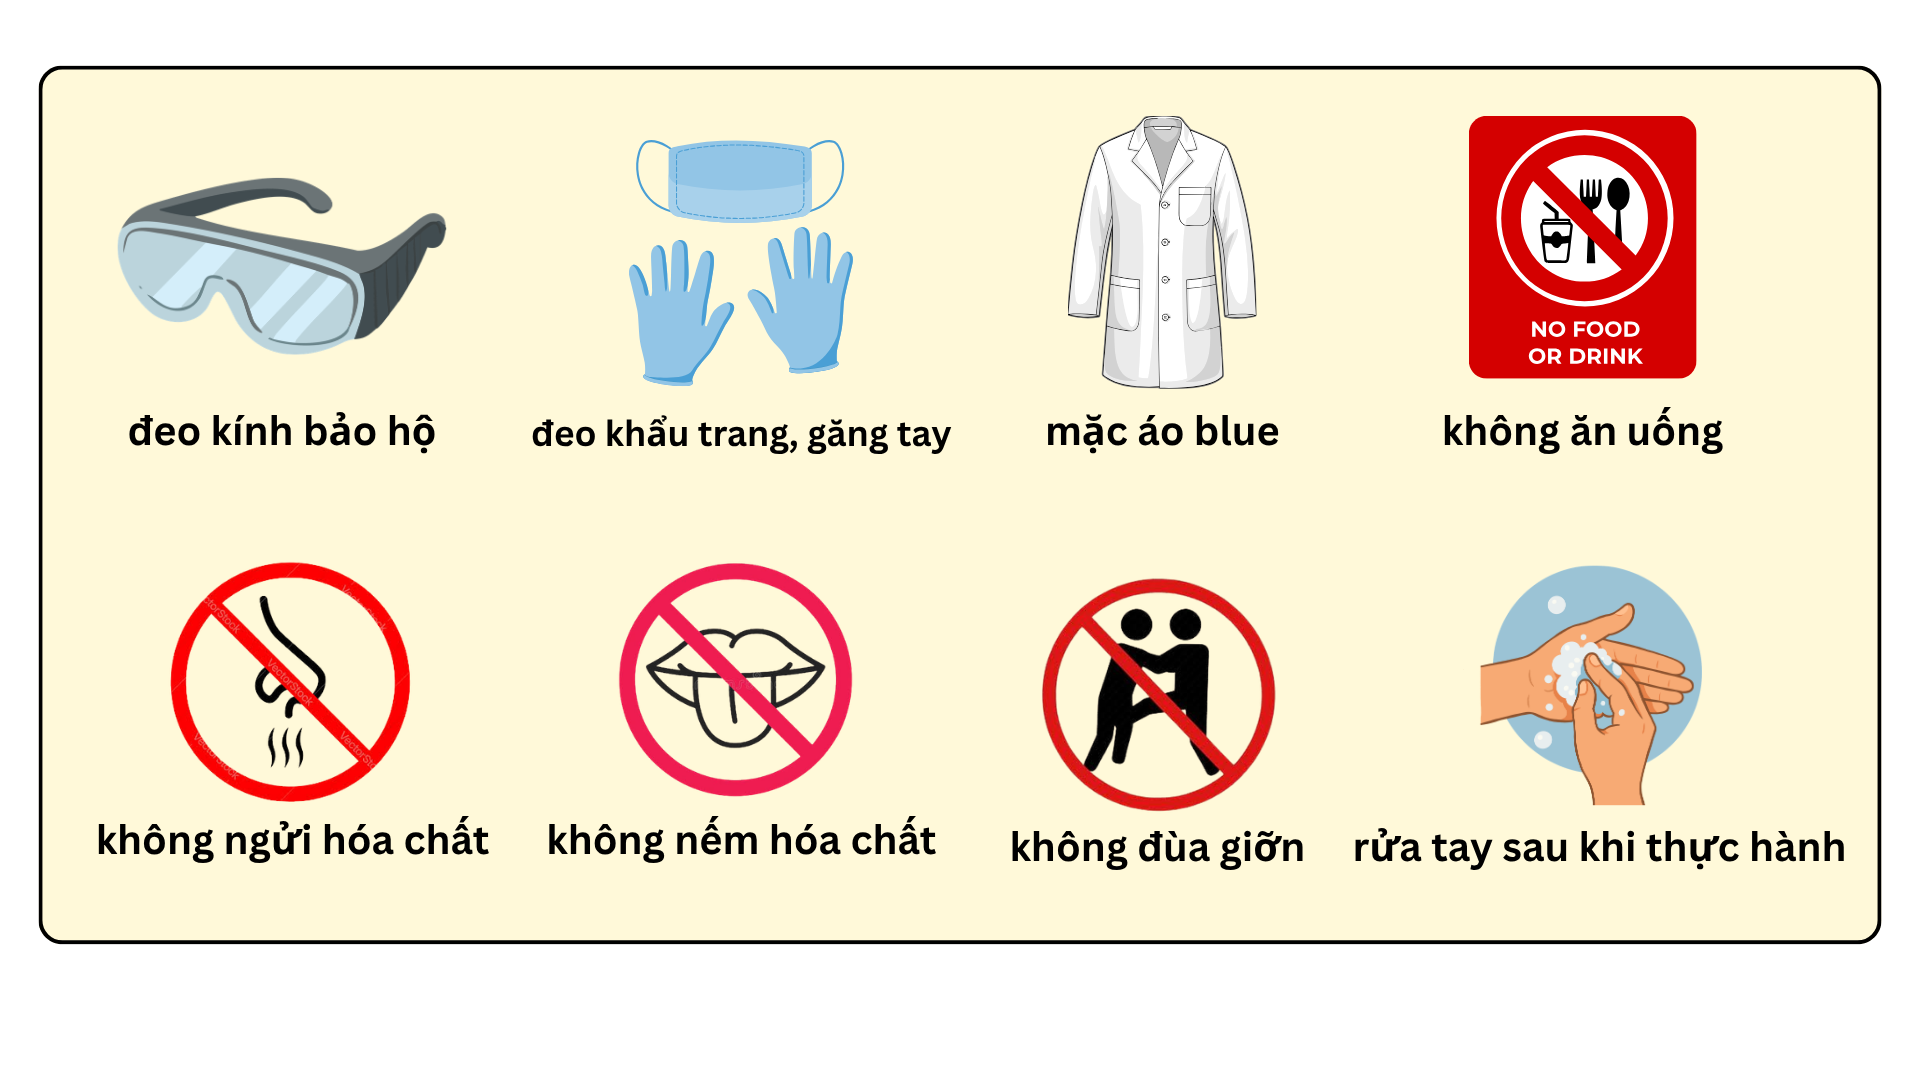
\includegraphics[width=0.98\linewidth,trim=1cm 3cm 1cmmm 1.5cm, clip ]{Images/DE_CUONG_HOA_6_HKI/quy_dinh_an_toan.png}
		\captionof{figure}{\textbf{\textit{Một số quy đinh an toàn trong phòng thí nghiệm}} }
		\end{center}
		Một số quy đinh an toàn trong phòng thí nghiệm:
		\begin{enumerate}
			\item Đọc kĩ hướng dẫn, nội quy và các kí hiệu cảnh báo trước khi làm thí nghiệm.
			\item Mặc trang phục gọn gàng; sử dụng kính, găng tay, áo bảo hộ khi cần.
			\item Không ăn uống, đùa nghịch; không tự ý nếm hoặc ngửi trực tiếp hoá chất.
			\item Thực hiện thí nghiệm theo hướng dẫn của giáo viên; báo ngay khi có sự cố.
			\item Thu gom chất thải đúng nơi quy định, dọn dẹp và rửa tay sau khi thực hành.
		\end{enumerate}
		\begin{ghinho}
			Luôn tuân thủ nội quy an toàn phòng thực hành và nhận diện đúng các kí hiệu cảnh báo trước khi tiến hành thí nghiệm.
		\end{ghinho}
	\end{kienthuccannho}
	\subsection{Bài tập}
	\phan{Bài tập tự luận}
	\Opensolutionfile{ansbth}[Ans/LGBT-C01_B02_AN_TOAN_TRONG_PHONG_THUC_HANH]
	\Opensolutionfile{ansbt}[Ans/AnsBT-C01_B02_AN_TOAN_TRONG_PHONG_THUC_HANH]
	%%%=============BT_1=============%%%
	\begin{bt}
		Vì sao trước khi tiến hành thí nghiệm, học sinh cần đọc kĩ các kí hiệu cảnh báo trên nhãn hoá chất, dụng cụ?
		\loigiai{
			Để nhận biết mức độ nguy hiểm như dễ cháy, ăn mòn, độc hại, ... của hoá chất hoặc dụng cụ, từ đó có biện pháp phòng tránh và sử dụng an toàn, tránh xảy ra tai nạn.
		}
	\end{bt}
	%%%=============BT_2=============%%%
	\begin{bt}
		Nêu $3$ quy định an toàn cần tuân thủ khi ở trong phòng thực hành.
		\loigiai{
			Có thể nêu $3$ quy định an toàn sau:
			\begin{enumerate}
				\item Không ăn uống, đùa nghịch trong phòng thực hành.
				\item Mặc đồ bảo hộ như kính, găng tay khi cần thiết.
				\item Không tự ý ngửi hoặc nếm hoá chất.
			\end{enumerate}
		}
	\end{bt}
	%%%=============BT_3=============%%%
	\begin{bt}
		Khi không may làm đổ hoá chất ra bàn thí nghiệm, em cần làm gì?
		\loigiai{
			Khi không may làm đổ hoá chất ra bàn thí nghiệm, em cần:
			\begin{enumerate}
				\item Báo ngay cho giáo viên.
				\item Không tự ý xử lí nếu chưa có hướng dẫn.
				\item Tránh tiếp xúc trực tiếp với hoá chất.
				\item Thực hiện đúng hướng dẫn xử lí sự cố của giáo viên.
			\end{enumerate}
		}
	\end{bt}
	%%%=============BT_4=============%%%
	\begin{bt}
		Em hãy nêu cách sử dụng bình chia độ để đo thể tích một lượng nước.
		\loigiai{
			Để đo thể tích một lượng nước bằng bình chia độ, em thực hiện:
			\begin{enumerate}
				\item Đặt bình chia độ trên mặt phẳng nằm ngang.
				\item Rót nước vào bình chia độ.
				\item Đặt mắt ngang với mực chất lỏng trong bình.
				\item Đọc và ghi kết quả theo vạch chia gần nhất với mực chất lỏng.
			\end{enumerate}
		}
	\end{bt}
	%%%=============BT_5=============%%%
	\begin{bt}
		Vì sao cần rửa tay sau khi làm thí nghiệm dù không tiếp xúc trực tiếp với hoá chất?
		\loigiai{
			Vì tay có thể dính hoá chất ở dạng hơi, bụi hoặc tiếp xúc gián tiếp qua dụng cụ, bàn thí nghiệm. Rửa tay giúp loại bỏ nguy cơ ảnh hưởng đến sức khoẻ.
		}
	\end{bt}
	%%%=============BT_6=============%%%
	\begin{bt}
		Kể tên $2$ kí hiệu cảnh báo em thường gặp trong phòng thực hành và nêu ý nghĩa của chúng.
		\loigiai{
			Có thể nêu:
			\begin{enumerate}
				\item Kí hiệu chất dễ cháy: cảnh báo chất có khả năng bắt cháy, cần tránh xa nguồn lửa và nguồn nhiệt.
				\item Kí hiệu chất độc: cảnh báo chất gây hại cho sức khoẻ nếu tiếp xúc, hít phải hoặc nuốt phải.
			\end{enumerate}
		}
	\end{bt}
	%%%=============BT_7=============%%%
	\begin{bt}
		Trong phòng thí nghiệm ở trường, em thấy trên tủ đựng hoá chất có dán nhãn hình ngọn lửa như hình vẽ. Nếu vô tình phải làm việc gần khu vực này, em cần lưu ý điều gì để đảm bảo an toàn?
		\begin{center}
		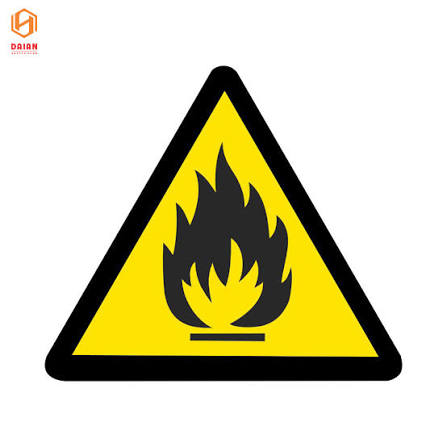
\includegraphics[width=0.26\linewidth,trim=1.5cm 2.0cm 1.5cm 2.2cm, clip]{Images/DE_CUONG_HOA_6_HKI/chat_de_chay_1.jpg}
		\end{center}
		\loigiai{
			Đây là kí hiệu cảnh báo chất dễ cháy. Khi làm việc gần khu vực này, em cần:
			\begin{enumerate}
				\item Tránh xa nguồn lửa và nguồn nhiệt.
				\item Không hút thuốc, không dùng bật lửa hoặc diêm gần khu vực đó.
				\item Báo giáo viên nếu phát hiện mùi lạ hoặc dấu hiệu bất thường.
			\end{enumerate}
		}
	\end{bt}
	%%%=============BT_8=============%%%
	\begin{bt}
		Em hãy nêu $3$ việc cần làm khi phát hiện một bạn trong lớp không tuân thủ quy định an toàn trong phòng thực hành (ví dụ: định nếm thử hoá chất lạ).
		\loigiai{
			Có thể nêu $3$ việc cần làm:
			\begin{enumerate}
				\item Ngăn bạn lại ngay.
				\item Giải thích nguy cơ của việc làm đó.
				\item Báo ngay cho giáo viên để được hướng dẫn xử lí.
			\end{enumerate}
		}
	\end{bt}
	%%%=============BT_9=============%%%
	\begin{bt}
		Vì sao các kí hiệu cảnh báo trên hoá chất thường được thiết kế bằng hình ảnh, màu sắc dễ nhận biết thay vì chỉ ghi chữ?
		\loigiai{
			Vì hình ảnh và màu sắc giúp nhận biết nhanh, trực quan, không phụ thuộc hoàn toàn vào khả năng đọc chữ hay ngôn ngữ, nhờ đó mọi người dễ nhận ra mức độ nguy hiểm để phòng tránh kịp thời.
		}
	\end{bt}
	%%%=============BT_10=============%%%
	\begin{bt}
		Ở nhà, khi sử dụng các sản phẩm tẩy rửa có ghi kí hiệu cảnh báo (ví dụ: chất ăn mòn, chất độc hại), em cần lưu ý điều gì để đảm bảo an toàn cho bản thân và gia đình?
		\loigiai{
			Khi sử dụng các sản phẩm tẩy rửa có kí hiệu cảnh báo, em cần:
			\begin{enumerate}
				\item Đọc kĩ nhãn và kí hiệu cảnh báo trước khi dùng.
				\item Đeo găng tay nếu cần tiếp xúc.
				\item Không trộn lẫn các loại hoá chất tẩy rửa khác nhau nếu không có hướng dẫn.
				\item Để xa tầm tay trẻ nhỏ.
				\item Rửa tay sạch sau khi sử dụng.
			\end{enumerate}
		}
	\end{bt}
	\Closesolutionfile{ansbt}
	\Closesolutionfile{ansbth}

	\phan{Bài tập trắc nghiệm nhiều lựa chọn}
	\textit{\large Thí sinh trả lời từ câu 1 đến câu 20. Mỗi câu thí sinh chỉ chọn một phương án}
	\Opensolutionfile{ansex}[Ans/LGEX-C01_B02_AN_TOAN_TRONG_PHONG_THUC_HANH]
	\Opensolutionfile{ans}[Ans/Ans-C01_B02_AN_TOAN_TRONG_PHONG_THUC_HANH]
	%%%=============EX_1=============%%%
	\begin{ex}
		\immini{Kí hiệu cảnh báo hình đầu lâu xương chéo thể hiện điều gì?
			\choice
			{Chất dễ cháy}
			{\True Chất độc}
			{Chất ăn mòn}
			{Nguy hiểm về điện}
			}{			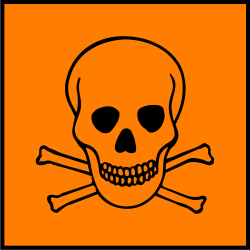
\includegraphics[width=0.2\linewidth]{Images/DE_CUONG_HOA_6_HKI/bien_bao_2.png}}
		\loigiai{Kí hiệu hình đầu lâu xương chéo dùng để cảnh báo chất độc, có thể gây hại cho sức khoẻ nếu tiếp xúc, hít phải hoặc nuốt phải.}
	\end{ex}
	%%%=============EX_2=============%%%
	\begin{ex}
		Kí hiệu cảnh báo hình ngọn lửa thể hiện điều gì?
		\begin{center}
			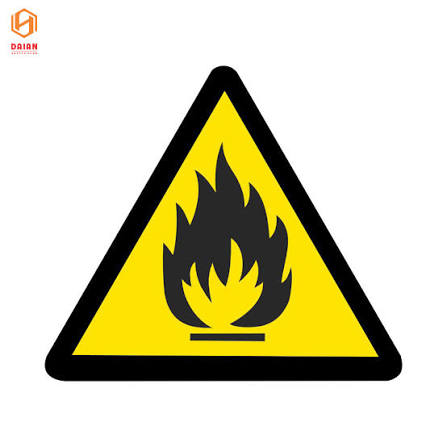
\includegraphics[width=0.26\linewidth,trim=1.5cm 2.0cm 1.5cm 1.5cm, clip]{Images/DE_CUONG_HOA_6_HKI/chat_de_chay_1.jpg}
		\end{center}
		\vspace*{-0.7cm}
		\choice
		{\True Chất dễ cháy}
		{Chất độc}
		{Chất phóng xạ}
		{Nguy hiểm sinh học}
		\loigiai{Kí hiệu hình ngọn lửa cảnh báo chất dễ cháy, cần tránh xa nguồn lửa và nguồn nhiệt.}
	\end{ex}
	%%%=============EX_3=============%%%
	\begin{ex}
		Trong phòng thực hành, học sinh không được phép làm gì?
		\choice
		{Đeo kính bảo hộ khi cần}
		{\True Ăn uống, đùa nghịch}
		{Rửa tay sau khi thí nghiệm}
		{Báo giáo viên khi có sự cố}
		\loigiai{Ăn uống, đùa nghịch trong phòng thực hành dễ gây mất an toàn nên là việc không được phép làm.}
	\end{ex}
	%%%=============EX_4=============%%%
	\begin{ex}
		Vì sao không nên tự ý nếm hoặc ngửi trực tiếp hoá chất trong phòng thực hành?
		\choice
		{\True Vì hoá chất có thể độc hại, gây nguy hiểm cho sức khoẻ}
		{Vì hoá chất luôn có mùi khó chịu}
		{Vì làm vậy tốn hoá chất}
		{Vì quy định không cho phép quan sát hoá chất}
		\loigiai{Hoá chất có thể độc hại, gây bỏng, ngộ độc hoặc ảnh hưởng đến đường hô hấp nên không được nếm hoặc ngửi trực tiếp.}
	\end{ex}
	%%%=============EX_5=============%%%
	\begin{ex}
		Việc nhận biết đúng các kí hiệu cảnh báo trong phòng thực hành giúp ích gì?
		\choice
		{Giúp trang trí phòng thí nghiệm đẹp hơn}
		{\True Giúp nhận biết mức độ nguy hiểm và có biện pháp phòng tránh phù hợp}
		{Giúp tiết kiệm hoá chất}
		{Không có tác dụng gì đặc biệt}
		\loigiai{Nhận biết đúng kí hiệu cảnh báo giúp học sinh biết trước nguy cơ để sử dụng dụng cụ, hoá chất an toàn hơn.}
	\end{ex}
	%%%=============EX_6=============%%%
	\begin{ex}
		Nếu không may hoá chất bắn vào mắt, việc đầu tiên cần làm là gì?
		\choice
		{Dụi mắt thật mạnh}
		{\True Rửa ngay bằng nước sạch nhiều lần và báo giáo viên}
		{Tiếp tục thí nghiệm bình thường}
		{Uống nước để giảm đau}
		\loigiai{Khi hoá chất bắn vào mắt cần rửa ngay bằng nước sạch nhiều lần để giảm tác hại, sau đó báo ngay cho giáo viên để được hỗ trợ.}
	\end{ex}
	%%%=============EX_7=============%%%
	\begin{ex}
		Việc nào sau đây là việc nên làm trong phòng thực hành?
		\choice
		{Mang đồ ăn vào phòng thực hành}
		{\True Buộc tóc gọn gàng khi làm thí nghiệm}
		{Mang hết các đồ thí nghiệm ra bàn thực hành}
		{Đổ hoá chất vào cống thoát nước}
		\loigiai{Buộc tóc gọn gàng giúp tránh tóc vướng vào lửa, hoá chất hoặc dụng cụ thí nghiệm nên là việc nên làm.}
	\end{ex}
	%%%=============EX_8=============%%%
	\begin{ex}
		Để đảm bảo an toàn trong phòng thực hành cần thực hiện nguyên tắc nào dưới đây?
		\choice
		{Làm thí nghiệm theo sự hướng dẫn của bạn bè trong lớp}
		{Có thể nhận biết hoá chất bằng cách ngửi hoá chất}
		{Mang đồ ăn vào phòng thực hành}
		{\True Đọc kĩ nội quy và thực hiện theo nội quy phòng thực hành}
		\loigiai{Đọc kĩ nội quy và thực hiện đúng nội quy là nguyên tắc cơ bản để đảm bảo an toàn trong phòng thực hành.}
	\end{ex}
	%%%=============EX_9=============%%%
	\begin{ex}
		Trong phòng thực hành có dán kí hiệu cảnh báo chất ăn mòn. Học sinh cần làm gì khi làm việc gần khu vực đó?
		\choice
		{Có thể chạm tay trực tiếp vì chỉ là kí hiệu}
		{\True Đeo găng tay, kính bảo hộ và tránh để hoá chất tiếp xúc với da}
		{Không cần chú ý gì đặc biệt}
		{Chỉ cần đứng xa $10$ m là an toàn tuyệt đối}
		\loigiai{Kí hiệu chất ăn mòn cảnh báo nguy cơ gây bỏng da, hỏng quần áo hoặc tổn thương mắt nên cần dùng đồ bảo hộ và tránh tiếp xúc trực tiếp.}
	\end{ex}
	%%%=============EX_10=============%%%
	\begin{ex}
		Vì sao các quy định an toàn trong phòng thực hành môn Khoa học tự nhiên đặc biệt quan trọng?
		\choice
		{\True Vì phòng thực hành có sử dụng dụng cụ, hoá chất, thiết bị có thể gây nguy hiểm nếu không tuân thủ đúng quy định}
		{Vì phòng thực hành lúc nào cũng đông người}
		{Vì môn Khoa học tự nhiên khó hơn các môn khác}
		{Vì phòng thực hành không có giáo viên giám sát}
		\loigiai{Phòng thực hành có nhiều dụng cụ, thiết bị và hoá chất tiềm ẩn nguy hiểm nên phải tuân thủ nghiêm các quy định an toàn.}
	\end{ex}
	%%%=============EX_11=============%%%
	\begin{ex}
		Cho các việc làm: (a) đeo găng tay khi tiếp xúc hoá chất; (b) nếm thử hoá chất lạ để nhận biết; (c) đọc kĩ nhãn và kí hiệu cảnh báo trước khi dùng hoá chất; (d) đổ hoá chất thừa trở lại lọ chứa ban đầu. Số việc làm đúng theo quy định an toàn là
		\choice
		{1}
		{\True 2}
		{3}
		{4}
		\loigiai{Các việc làm đúng là (a) và (c). Việc (b) sai vì không được nếm hoá chất lạ. Việc (d) sai vì có thể làm nhiễm bẩn lọ hoá chất ban đầu.}
	\end{ex}
	%%%=============EX_12=============%%%
	\begin{ex}
		Hoạt động nào sau đây không thực hiện đúng quy tắc an toàn trong phòng thực hành?
		\choice
		{Đeo găng tay khi làm thí nghiệm}
		{Không ăn uống, đùa nghịch trong phòng thí nghiệm}
		{\True Để hoá chất không đúng nơi quy định sau khi làm xong thí nghiệm}
		{Làm thí nghiệm theo sự hướng dẫn của giáo viên}
		\loigiai{Hoá chất sau khi dùng phải được đặt lại đúng nơi quy định để tránh nhầm lẫn, đổ vỡ hoặc gây nguy hiểm cho người khác.}
	\end{ex}
	%%%=============EX_13=============%%%
	\begin{ex}
		Biển báo trong hình dưới đây có ý nghĩa gì?
		\begin{center}
		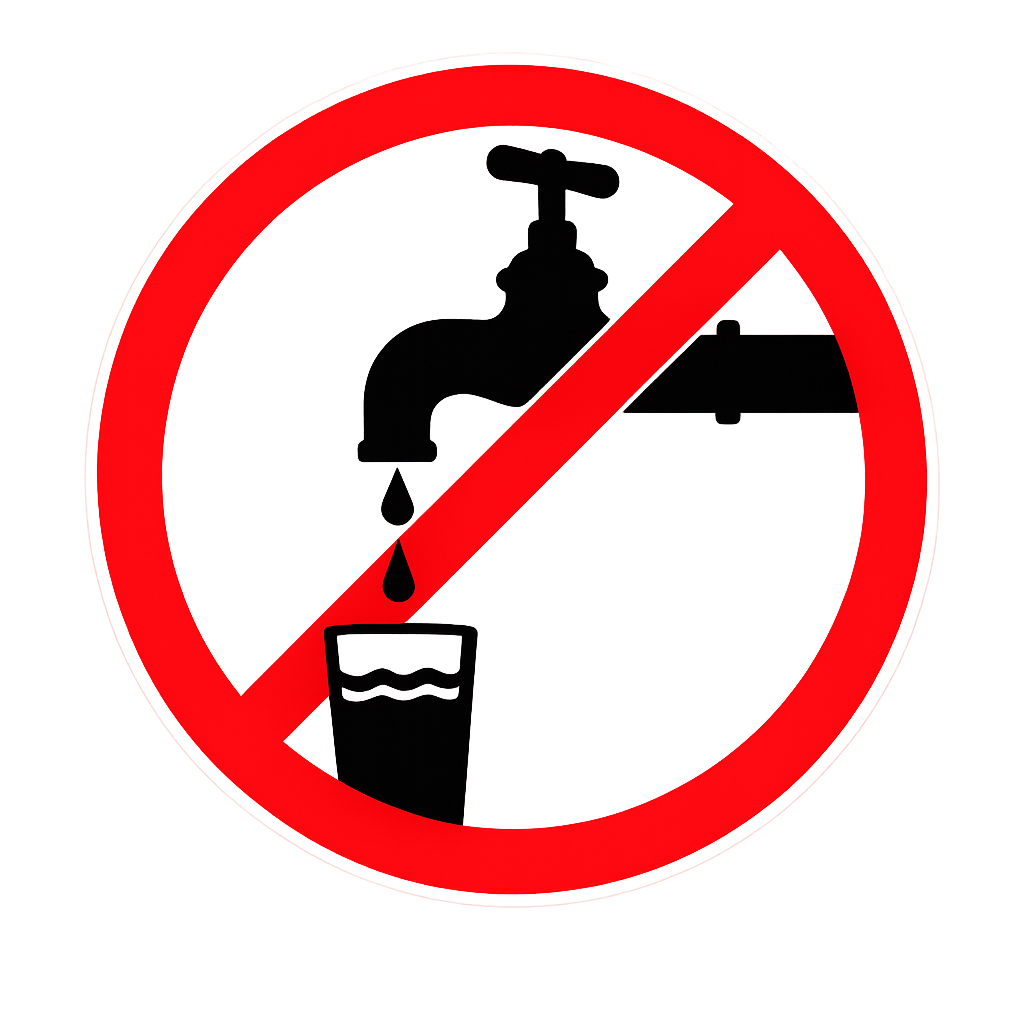
\includegraphics[width=0.20\linewidth,trim=1.5cm 3.0cm 1.5cm 0.8cm, clip]{Images/DE_CUONG_HOA_6_HKI/cam_su_dung_nuoc.png}
		\end{center}
		\vspace*{-1cm}
		\choice
		{\True Cấm uống nước}
		{Cấm lửa}
		{Chất độc sinh học}
		{Chất ăn mòn}
		\loigiai{Biển báo có hình cốc nước bị gạch chéo thể hiện nội dung cấm uống nước hoặc cấm ăn uống tại khu vực đó.}
	\end{ex}
	%%%=============EX_14=============%%%
	\begin{ex}
		Khi làm thí nghiệm, không may làm vỡ ống hoá chất xuống sàn nhà, ta cần phải làm gì đầu tiên?
		\choice
		{Lấy tay hót hoá chất bị đổ vào ống hoá chất khác}
		{Dùng tay nhặt ống hoá chất đã vỡ vào thùng rác}
		{\True Báo ngay cho giáo viên và thực hiện theo hướng dẫn xử lí sự cố}
		{Gọi cấp cứu y tế ngay lập tức trong mọi trường hợp}
		\loigiai{Khi làm vỡ ống hoá chất cần báo ngay cho giáo viên để được hướng dẫn xử lí đúng cách, tránh tự ý chạm vào hoá chất hoặc mảnh vỡ.}
	\end{ex}
	%%%=============EX_15=============%%%
	\begin{ex}
		Biển báo dưới đây có ý nghĩa gì?
		\begin{center}
		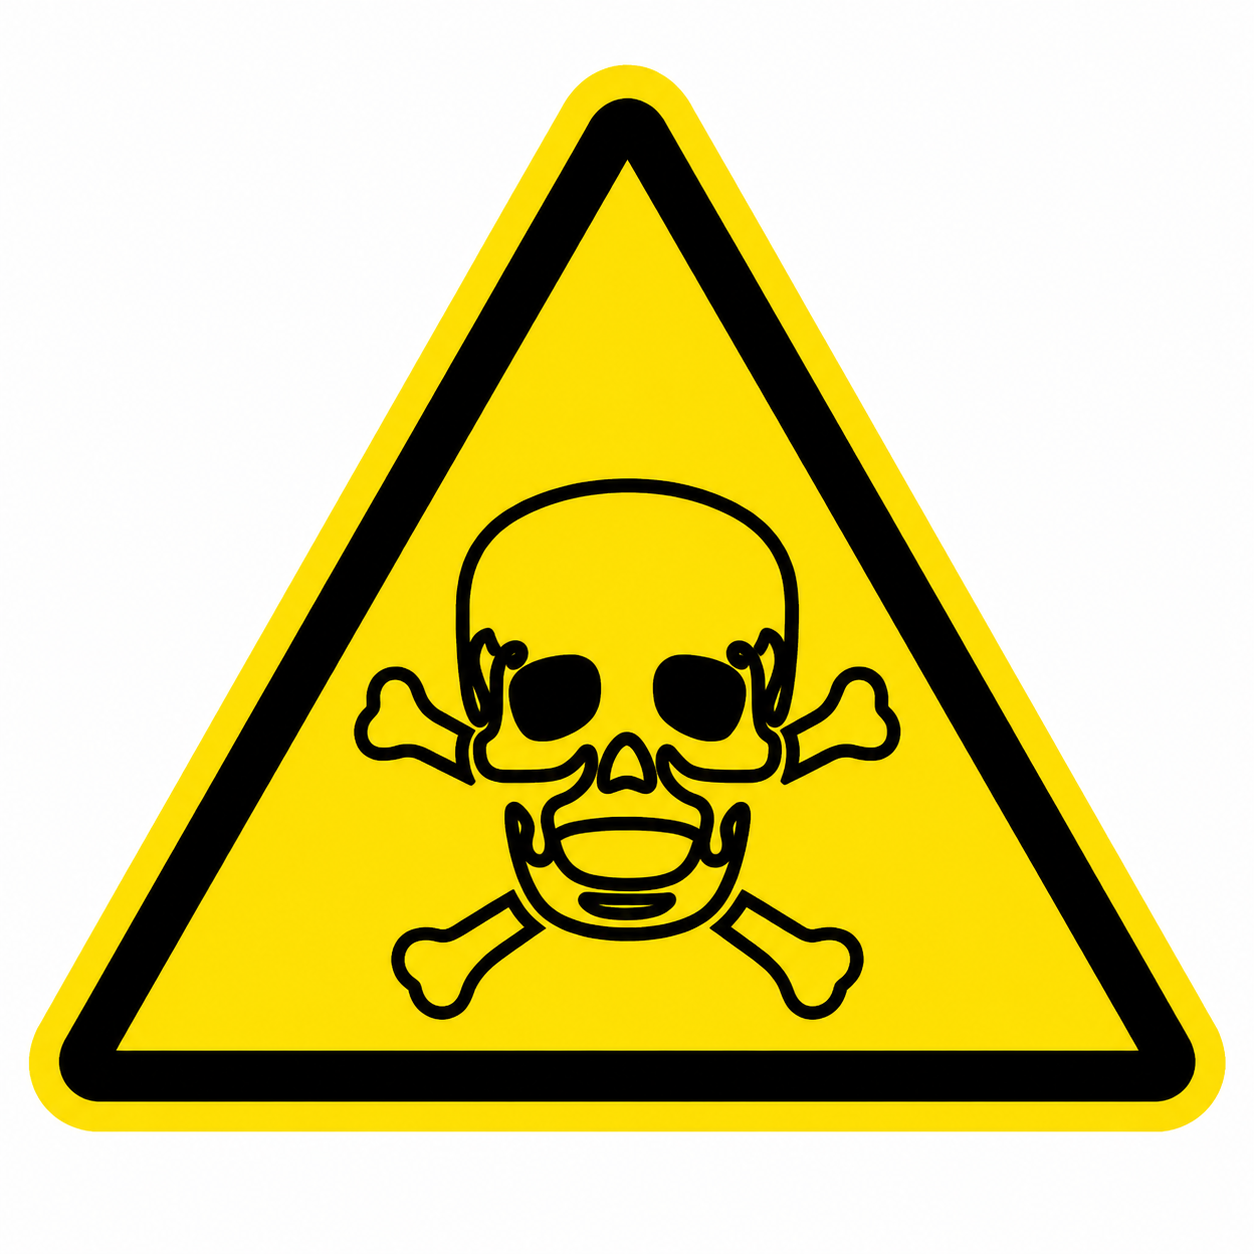
\includegraphics[width=0.2\linewidth,trim=1.5cm 3.0cm 1.5cm 0.8cm, clip]{Images/DE_CUONG_HOA_6_HKI/khu_vuc_nguy_hiem.png}
		\end{center}
		\vspace*{-0.7cm}
		\choice
		{Cấm thực hiện}
		{\True Cảnh báo các khu vực nguy hiểm }
		{Cảnh báo chỉ dẫn thực hiện}
		{Cảnh báo chất độc}
		\loigiai{Biển báo có hình đầu lâu xương chéo là kí hiệu cảnh báo các khu vực nguy hiểm.}
	\end{ex}
	%%%=============EX_16=============%%%
	\begin{ex}
		Vì sao cần tuân thủ các kí hiệu cảnh báo trên nhãn hoá chất trước khi tiến hành thí nghiệm, thay vì chỉ xem sau khi có sự cố?
		\choice
		{\True Vì kí hiệu cảnh báo giúp nhận biết trước mức độ nguy hiểm để chủ động phòng tránh tai nạn}
		{Vì quy định bắt buộc phải đọc trước cho có hình thức}
		{Vì đọc trước giúp tiết kiệm hoá chất}
		{Vì kí hiệu chỉ có tác dụng sau khi xảy ra sự cố}
		\loigiai{Kí hiệu cảnh báo giúp người thực hành biết trước nguy cơ để lựa chọn cách thao tác, bảo hộ và phòng tránh phù hợp ngay từ đầu.}
	\end{ex}
	%%%=============EX_17=============%%%
	\begin{ex}
		Trong phòng thực hành có dán kí hiệu cảnh báo chất ăn mòn. Học sinh cần làm gì khi làm việc gần khu vực đó?
		\choice
		{Có thể chạm tay trực tiếp vì chỉ là kí hiệu}
		{\True Đeo găng tay, kính bảo hộ và tránh để hoá chất tiếp xúc với da}
		{Không cần chú ý gì đặc biệt}
		{Chỉ cần đứng xa $10$ m là an toàn tuyệt đối}
		\loigiai{Khu vực có cảnh báo chất ăn mòn cần được thao tác cẩn thận, dùng bảo hộ và tránh tiếp xúc trực tiếp với hoá chất.}
	\end{ex}
	%%%=============EX_18=============%%%
	\begin{ex}
		Vì sao các quy định an toàn trong phòng thực hành môn Khoa học tự nhiên đặc biệt quan trọng?
		\choice
		{\True Vì phòng thực hành có sử dụng dụng cụ, hoá chất, thiết bị có thể gây nguy hiểm nếu không tuân thủ đúng quy định}
		{Vì phòng thực hành lúc nào cũng đông người}
		{Vì môn Khoa học tự nhiên khó hơn các môn khác}
		{Vì phòng thực hành không có giáo viên giám sát}
		\loigiai{Các quy định an toàn nhằm giảm nguy cơ tai nạn khi sử dụng hoá chất, dụng cụ thuỷ tinh, nguồn nhiệt và thiết bị điện trong phòng thực hành.}
	\end{ex}
	%%%=============EX_19=============%%%
	\begin{ex}
		Cho các việc làm: (a) đeo găng tay khi tiếp xúc hoá chất; (b) nếm thử hoá chất lạ để nhận biết; (c) đọc kĩ nhãn và kí hiệu cảnh báo trước khi dùng hoá chất; (d) đổ hoá chất thừa trở lại lọ chứa ban đầu. Số việc làm đúng theo quy định an toàn là
		\choice
		{1}
		{\True 2}
		{3}
		{4}
		\loigiai{Có $2$ việc làm đúng là (a) và (c). Hai việc còn lại vi phạm quy tắc an toàn trong phòng thực hành.}
	\end{ex}
	%%%=============EX_20=============%%%
	\begin{ex}
		Khi làm việc gần tủ hoá chất có dán kí hiệu cảnh báo chất dễ cháy, nhóm học sinh cần lưu ý điều gì?
		\choice
		{Có thể mang bật lửa, diêm lại gần vì chỉ là kí hiệu}
		{\True Tránh xa nguồn lửa, nguồn nhiệt, không hút thuốc hay dùng lửa gần khu vực đó}
		{Không cần lưu ý gì đặc biệt}
		{Chỉ nguy hiểm nếu chạm trực tiếp vào tủ}
		\loigiai{Kí hiệu chất dễ cháy cho biết khu vực đó có nguy cơ bắt lửa cao nên phải tránh mọi nguồn gây cháy.}
	\end{ex}
	\Closesolutionfile{ans}
	\Closesolutionfile{ansex}

	\phan{Bài tập trắc nghiệm đúng sai}
	\textit{\large Thí sinh trả lời từ câu 1 đến câu 12. Trong mỗi ý a), b), c), d) ở mỗi câu thí sinh chọn đúng hoặc sai}
	\Opensolutionfile{ansex}[Ans/LGTF-C01_B02_AN_TOAN_TRONG_PHONG_THUC_HANH]
	\Opensolutionfile{ansbook}[Ansbook/AnsTF-C01_B02_AN_TOAN_TRONG_PHONG_THUC_HANH]
	\Opensolutionfile{ans}[Ans/Tempt-C01_B02_AN_TOAN_TRONG_PHONG_THUC_HANH]
	\setcounter{ex}{0}
	%%%=============TF_1=============%%%
	\begin{ex}
		Về an toàn trong phòng thực hành, đánh giá các phát biểu sau:
		\choiceTF
		{Có thể nếm thử hoá chất lạ với lượng rất nhỏ để nhận biết}
		{\True Kí hiệu hình ngọn lửa cảnh báo chất dễ cháy}
		{\True Cần rửa tay sau khi làm thí nghiệm dù đã đeo găng tay}
		{Khi làm đổ hoá chất, học sinh nên tự xử lí ngay để tiết kiệm thời gian}
		\loigiai{
			\begin{itemchoice}[F1,T2,T3,F4]
				\itemch Không được nếm thử hoá chất lạ vì có thể gây ngộ độc hoặc bỏng.
				\itemch Hình ngọn lửa là kí hiệu cảnh báo chất dễ cháy nên phát biểu đúng.
				\itemch Sau thí nghiệm vẫn cần rửa tay để loại bỏ hoá chất có thể bám gián tiếp nên phát biểu đúng.
				\itemch Khi làm đổ hoá chất cần báo giáo viên và xử lí theo hướng dẫn, không tự ý làm nên phát biểu sai.
			\end{itemchoice}
		}
	\end{ex}
	%%%=============TF_2=============%%%
	\begin{ex}
		Xét về an toàn trong phòng thực hành, đánh giá các phát biểu sau:
		\choiceTF
		{\True Cần đeo kính hoặc găng tay bảo hộ khi cần thiết}
		{Có thể tự ý ngửi hoá chất lạ nếu thấy tò mò}
		{\True Kí hiệu cảnh báo trên nhãn hoá chất giúp nhận biết mức độ nguy hiểm}
		{Không cần báo giáo viên khi làm đổ hoá chất, có thể tự xử lí}
		\loigiai{
			\begin{itemchoice}[T1,F2,T3,F4]
				\itemch Kính và găng tay bảo hộ giúp giảm nguy cơ tiếp xúc với hoá chất nên phát biểu đúng.
				\itemch Tự ý ngửi hoá chất lạ là nguy hiểm nên phát biểu sai.
				\itemch Kí hiệu cảnh báo cho biết nguy cơ của hoá chất nên phát biểu đúng.
				\itemch Làm đổ hoá chất phải báo giáo viên để xử lí an toàn nên phát biểu sai.
			\end{itemchoice}
		}
	\end{ex}
	%%%=============TF_3=============%%%
	\begin{ex}
		Trong phòng thực hành có dán đồng thời hai kí hiệu cảnh báo chất độc và chất dễ cháy trên một tủ đựng hoá chất. Đánh giá các phát biểu sau:
		\choiceTF
		{\True Học sinh cần tránh tiếp xúc trực tiếp và tránh mang nguồn lửa đến gần tủ này}
		{Chỉ cần lưu ý một trong hai kí hiệu là đủ}
		{\True Việc dán đồng thời hai kí hiệu cho thấy hoá chất trong tủ có thể gây nguy hiểm theo nhiều cách khác nhau}
		{Có thể mở tủ và tiếp xúc bình thường vì đã có kí hiệu cảnh báo dán sẵn}
		\loigiai{
			\begin{itemchoice}[T1,F2,T3,F4]
				\itemch Tủ vừa có chất độc vừa có chất dễ cháy nên phải tránh tiếp xúc và tránh nguồn lửa; phát biểu đúng.
				\itemch Cần chú ý đầy đủ mọi kí hiệu cảnh báo nên phát biểu sai.
				\itemch Nhiều kí hiệu cho thấy có nhiều loại nguy cơ khác nhau nên phát biểu đúng.
				\itemch Có kí hiệu cảnh báo không có nghĩa là được tiếp xúc bình thường; phát biểu sai.
			\end{itemchoice}
		}
	\end{ex}
	%%%=============TF_4=============%%%
	\begin{ex}
		Trong phòng thực hành, trên một tủ hoá chất có dán đồng thời hai kí hiệu cảnh báo chất ăn mòn và chất dễ cháy. Đánh giá các phát biểu sau:
		\choiceTF
		{\True Học sinh cần đeo găng tay, kính bảo hộ khi thao tác gần khu vực này}
		{Có thể mang bật lửa, diêm đến gần khu vực này vì hai kí hiệu không liên quan đến nhau}
		{\True Việc nhận biết đúng các kí hiệu cảnh báo giúp phòng tránh tai nạn trước khi thao tác}
		{Chỉ cần quan tâm đến kí hiệu cảnh báo sau khi sự cố đã xảy ra}
		\loigiai{
			\begin{itemchoice}[T1,F2,T3,F4]
				\itemch Chất ăn mòn có thể gây hại cho da, mắt nên cần đeo bảo hộ; phát biểu đúng.
				\itemch Khu vực có chất dễ cháy phải tránh nguồn lửa nên phát biểu sai.
				\itemch Nhận biết đúng kí hiệu cảnh báo giúp chủ động phòng tránh nên phát biểu đúng.
				\itemch Phải quan tâm đến kí hiệu cảnh báo trước khi thao tác chứ không chờ sự cố xảy ra; phát biểu sai.
			\end{itemchoice}
		}
	\end{ex}
	%%%=============TF_5=============%%%
	\begin{ex}
		Một phòng thí nghiệm hoá học ở trường học có dán các kí hiệu cảnh báo trên tủ đựng hoá chất và yêu cầu học sinh mặc áo bảo hộ khi thực hành. Đánh giá các phát biểu sau:
		\choiceTF
		{\True Việc dán kí hiệu cảnh báo giúp học sinh nhận biết nguy cơ trước khi thao tác với hoá chất}
		{\True Mặc áo bảo hộ là biện pháp giúp hạn chế hoá chất tiếp xúc trực tiếp với da, quần áo}
		{Những quy định này không cần thiết nếu học sinh cẩn thận}
		{Nếu không có kí hiệu cảnh báo thì hoá chất chắc chắn không nguy hiểm}
		\loigiai{
			\begin{itemchoice}[T1,T2,F3,F4]
				\itemch Kí hiệu cảnh báo giúp nhận biết trước nguy cơ của hoá chất nên phát biểu đúng.
				\itemch Áo bảo hộ giúp giảm nguy cơ hoá chất bám lên cơ thể và quần áo nên phát biểu đúng.
				\itemch Dù cẩn thận vẫn cần tuân thủ quy định an toàn nên phát biểu sai.
				\itemch Có những hoá chất nguy hiểm nhưng không thể chủ quan chỉ vì không nhìn thấy kí hiệu; phát biểu sai.
			\end{itemchoice}
		}
	\end{ex}
	%%%=============TF_6=============%%%
	\begin{ex}
		Một bạn học sinh cần đo thể tích của một viên đá cuội nhỏ, hình dạng không đều, không thấm nước. Đánh giá các phát biểu sau:
		\choiceTF
		{\True Có thể dùng bình chia độ chứa sẵn một lượng nước, thả viên đá vào và đo phần thể tích nước dâng lên để suy ra thể tích viên đá}
		{Có thể dùng thước thẳng đo trực tiếp và tính được thể tích chính xác vì viên đá có hình dạng không đều}
		{\True Phương pháp đo gián tiếp qua thể tích nước dâng lên áp dụng được cho các vật rắn không thấm nước, có hình dạng bất kì}
		{Không thể đo được thể tích của vật có hình dạng không đều bằng bất kì dụng cụ nào}
		\loigiai{
			\begin{itemchoice}[T1,F2,T3,F4]
				\itemch Đo phần nước dâng lên là cách xác định thể tích vật rắn không thấm nước; phát biểu đúng.
				\itemch Vật có hình dạng không đều không thể đo chính xác bằng thước thẳng đơn giản; phát biểu sai.
				\itemch Phương pháp dời chỗ của nước dùng được cho nhiều vật rắn không thấm nước nên phát biểu đúng.
				\itemch Vẫn có thể đo bằng bình chia độ nên phát biểu sai.
			\end{itemchoice}
		}
	\end{ex}
	%%%=============TF_7=============%%%
	\begin{ex}
		Trước khi tiến hành một thí nghiệm trong phòng thực hành, đánh giá các phát biểu sau:
		\choiceTF
		{\True Học sinh cần đọc kĩ hướng dẫn và chỉ tiến hành thí nghiệm khi có người hướng dẫn}
		{Có thể tự thay đổi các bước thí nghiệm nếu thấy cách khác nhanh hơn}
		{\True Cần nhận biết trước các vật liệu và nguồn có thể gây nguy hiểm}
		{Không cần quan tâm đến nhãn trên lọ hoá chất nếu đã từng sử dụng lọ đó}
		\loigiai{
			\begin{itemchoice}[T1,F2,T3,F4]
				\itemch Đọc hướng dẫn và làm theo người hướng dẫn giúp đảm bảo an toàn nên phát biểu đúng.
				\itemch Tự ý thay đổi quy trình có thể gây sự cố nên phát biểu sai.
				\itemch Nhận biết vật liệu nguy hiểm trước khi làm là việc cần thiết nên phát biểu đúng.
				\itemch Luôn phải đọc nhãn hoá chất trước khi dùng để tránh nhầm lẫn nên phát biểu sai.
			\end{itemchoice}
		}
	\end{ex}
	%%%=============TF_8=============%%%
	\begin{ex}
		Một nhóm học sinh chuẩn bị thực hành với hoá chất. Đánh giá các phát biểu sau:
		\choiceTF
		{\True Học sinh nên mặc trang phục gọn gàng và buộc tóc cao nếu tóc dài}
		{\True Kính bảo vệ mắt, găng tay và áo choàng có thể được sử dụng khi cần thiết}
		{Có thể đi lại, đùa nghịch trong lúc các bạn khác đang làm thí nghiệm}
		{\True Trang phục bảo hộ góp phần hạn chế nguy cơ hoá chất tiếp xúc với cơ thể}
		\loigiai{
			\begin{itemchoice}[T1,T2,F3,T4]
				\itemch Trang phục gọn gàng và buộc tóc giúp giảm nguy cơ vướng vào hoá chất hoặc lửa nên phát biểu đúng.
				\itemch Các phương tiện bảo hộ cá nhân cần dùng khi cần thiết nên phát biểu đúng.
				\itemch Đi lại, đùa nghịch trong phòng thực hành là không an toàn nên phát biểu sai.
				\itemch Trang phục bảo hộ giúp hạn chế hoá chất tiếp xúc trực tiếp với cơ thể nên phát biểu đúng.
			\end{itemchoice}
		}
	\end{ex}
	%%%=============TF_9=============%%%
	\begin{ex}
		Trong quá trình thực hành, một học sinh phát hiện dụng cụ thuỷ tinh bị nứt. Đánh giá các phát biểu sau:
		\choiceTF
		{\True Học sinh cần báo ngay cho giáo viên hoặc người hướng dẫn}
		{Có thể tiếp tục sử dụng nếu vết nứt còn nhỏ}
		{\True Dụng cụ thuỷ tinh bị nứt có thể vỡ và gây thương tích}
		{Học sinh nên tự dùng tay không thu gom các mảnh thuỷ tinh vỡ}
		\loigiai{
			\begin{itemchoice}[T1,F2,T3,F4]
				\itemch Phát hiện dụng cụ nứt phải báo ngay để tránh tai nạn; phát biểu đúng.
				\itemch Dụng cụ nứt không được tiếp tục sử dụng vì có thể vỡ bất ngờ; phát biểu sai.
				\itemch Thuỷ tinh bị nứt dễ vỡ và gây đứt tay nên phát biểu đúng.
				\itemch Không được dùng tay không nhặt mảnh vỡ vì rất nguy hiểm; phát biểu sai.
			\end{itemchoice}
		}
	\end{ex}
	%%%=============TF_10=============%%%
	\begin{ex}
		Một lọ hoá chất có dán kí hiệu hình đầu lâu và xương chéo. Đánh giá các phát biểu sau:
		\choiceTF
		{\True Kí hiệu này cảnh báo chất độc}
		{Có thể nếm một lượng rất nhỏ để kiểm tra chất có độc hay không}
		{\True Cần tránh để hoá chất tiếp xúc trực tiếp với cơ thể}
		{\True Cần tách biệt lọ hoá chất này ở khu vực riêng biệt với các lọ hoá chất khác}
		\loigiai{
			\begin{itemchoice}[T1,F2,T3,T4]
				\itemch Hình đầu lâu xương chéo là kí hiệu chất độc nên phát biểu đúng.
				\itemch Không được nếm thử bất kì hoá chất nào để kiểm tra nên phát biểu sai.
				\itemch Chất độc cần tránh tiếp xúc trực tiếp với cơ thể nên phát biểu đúng.
				\itemch Chất độc cần được bảo quản cẩn thận, tách biệt và có cảnh báo rõ ràng nên phát biểu đúng.
			\end{itemchoice}
		}
	\end{ex}
	%%%=============TF_11=============%%%
	\begin{ex}
		Một thiết bị trong phòng thực hành có gắn kí hiệu tia sét cảnh báo. Đánh giá các phát biểu sau:
		\choiceTF
		{\True Kí hiệu này cảnh báo nguy hiểm về điện}
		{Học sinh có thể tự ý tháo thiết bị để kiểm tra bên trong}
		{\True Cần tuân theo hướng dẫn khi sử dụng thiết bị có nguồn điện}
		{Có thể chạm vào thiết bị điện bằng tay ướt nếu thiết bị đang tắt}
		\loigiai{
			\begin{itemchoice}[T1,F2,T3,F4]
				\itemch Hình tia sét thường dùng để cảnh báo nguy hiểm về điện nên phát biểu đúng.
				\itemch Học sinh không được tự ý tháo thiết bị điện vì dễ gây mất an toàn; phát biểu sai.
				\itemch Thiết bị điện cần dùng đúng hướng dẫn để tránh tai nạn nên phát biểu đúng.
				\itemch Tay ướt vẫn có thể gây nguy hiểm khi tiếp xúc thiết bị điện nên phát biểu sai.
			\end{itemchoice}
		}
	\end{ex}
	%%%=============TF_12=============%%%
	\begin{ex}
		Trong một thí nghiệm, học sinh cần sử dụng dao và một số dụng cụ có đầu nhọn. Đánh giá các phát biểu sau:
		\choiceTF
		{\True Dao và dụng cụ sắc nhọn có thể gây thương tích nếu sử dụng không đúng cách}
		{\True Cần thao tác cẩn thận và thực hiện theo hướng dẫn của giáo viên}
		{Có thể dùng dụng cụ sắc nhọn để đùa nghịch khi chưa bắt đầu thí nghiệm}
		{\True Kí hiệu cảnh báo dụng cụ sắc nhọn giúp người thực hành nhận biết nguy cơ trước khi sử dụng}
		\loigiai{
			\begin{itemchoice}[T1,T2,F3,T4]
				\itemch Dụng cụ sắc nhọn có thể gây đâm, cắt nếu dùng sai cách nên phát biểu đúng.
				\itemch Thao tác cẩn thận và làm theo hướng dẫn là yêu cầu bắt buộc nên phát biểu đúng.
				\itemch Dùng dụng cụ sắc nhọn để đùa nghịch là rất nguy hiểm nên phát biểu sai.
				\itemch Kí hiệu cảnh báo giúp nhận biết trước nguy cơ để sử dụng an toàn hơn nên phát biểu đúng.
			\end{itemchoice}
		}
	\end{ex}
	\Closesolutionfile{ans}
	\Closesolutionfile{ansbook}
	\Closesolutionfile{ansex}

	\phan{Bài tập trả lời ngắn}
	\textit{\large Thí sinh trả lời từ câu 1 đến câu 7}
	\Opensolutionfile{ansex}[Ans/LGSA-C01_B02_AN_TOAN_TRONG_PHONG_THUC_HANH]
	\Opensolutionfile{ansexh}[Ans/AnsSA-C01_B02_AN_TOAN_TRONG_PHONG_THUC_HANH]
	\setcounter{ex}{0}
	%%%=============SA_1=============%%%
	\begin{ex}
		Một phòng thực hành dán $10$ kí hiệu cảnh báo, gồm: $4$ kí hiệu chất dễ cháy, $3$ kí hiệu chất độc, $2$ kí hiệu chất ăn mòn và $1$ kí hiệu nguy hiểm về điện. Có bao nhiêu kí hiệu liên quan trực tiếp đến hoá chất?
		\shortans{$9$}
		\loigiai{Các kí hiệu liên quan trực tiếp đến hoá chất là: chất dễ cháy ($4$), chất độc ($3$), chất ăn mòn ($2$). Tổng cộng là $4+3+2=9$.\\ \textbf{\textit{Đáp số:} $9$.}}
	\end{ex}
	%%%=============SA_2=============%%%
	\begin{ex}
		Trong các kí hiệu sau đây: 
		\begin{enumerate}[(1)]
			\item chất dễ cháy;
			\item chất độc;
			\item thuỷ tinh dễ vỡ;
			\item nhiệt độ cao;
			\item nguồn điện nguy hiểm.
		\end{enumerate}
		Có bao nhiêu kí hiệu cảnh báo liên quan trực tiếp đến hoá chất?
		\shortans{$2$}
		\loigiai{Các kí hiệu liên quan trực tiếp đến hoá chất là (1) chất dễ cháy và (2) chất độc. Vậy có $2$ kí hiệu.\\ \textbf{\textit{Đáp số:} $2$.}}
	\end{ex}
	%%%=============SA_3=============%%%
	\begin{ex}
		Trong các kí hiệu sau đây: 
		\begin{listEX}[3]
			\item[(1)] chất dễ cháy;
			\item[(2)] chất độc;
			\item[(3)] thuỷ tinh dễ vỡ;
			\item[(4)] nhiệt độ cao;
			\item[(5)] nguồn điện nguy hiểm.
		\end{listEX} 
		Có bao nhiêu kí hiệu cảnh báo liên quan trực tiếp đến hoá chất?
		\shortans{$2$}
		\loigiai{Trong danh sách đã cho, chỉ có (1) chất dễ cháy và (2) chất độc là kí hiệu liên quan trực tiếp đến hoá chất. Vậy có $2$ kí hiệu.\\ \textbf{\textit{Đáp số:} $2$.}}
	\end{ex}
	%%%=============SA_4=============%%%
	\begin{ex}
		Xét các việc làm sau: 
		\begin{enumerate}[(1)]
			\item mặc trang phục gọn gàng, nữ buộc tóc cao;
			\item đeo găng tay, khẩu trang, kính bảo vệ mắt khi cần; 
			\item tự ý tiến hành thí nghiệm khi chưa có người hướng dẫn;
			\item ăn uống, đùa nghịch trong phòng thí nghiệm;
			\item nhận biết vật liệu nguy hiểm trước khi làm thí nghiệm.
		\end{enumerate}
		Có bao nhiêu việc làm đúng quy định an toàn trong phòng thực hành?
		\shortans{$3$}
		\loigiai{Các việc làm đúng là (1), (2), (5). Hai việc (3), (4) vi phạm quy định an toàn. Vậy có $3$ việc làm đúng.\\ \textbf{\textit{Đáp số:} $3$.}}
	\end{ex}
	%%%=============SA_5=============%%%
	\begin{ex}
		Xét các việc làm sau khi kết thúc thí nghiệm: 
		\begin{listEX}[2]
			\item[(1)] thu gom chất thải để đúng nơi quy định;
			\item[(2)] lau dọn sạch sẽ chỗ làm việc;
			\item[(3)] sắp xếp dụng cụ gọn gàng, đúng chỗ;
			\item[(4)] rửa sạch tay bằng xà phòng;
			\item[(5)] đổ hoá chất thừa vào bồn rửa.
		\end{listEX} 
		Có bao nhiêu việc làm đúng quy định an toàn?
		\shortans{$4$}
		\loigiai{Các việc làm đúng là (1), (2), (3), (4). Việc (5) sai vì không được tự ý đổ hoá chất thừa vào bồn rửa. Vậy có $4$ việc làm đúng.\\ \textbf{\textit{Đáp số:} $4$.}}
	\end{ex}
	%%%=============SA_6=============%%%
	\begin{ex}
		Xét các tình huống sau: 
		\begin{enumerate}[(a)]
			\item thực hiện theo chỉ dẫn của giáo viên, báo cáo ngay khi thấy mối nguy hiểm;
			\item dùng tay kiểm tra mức độ nóng của vật khi đang đun; (c) ngửi hoặc nếm để tìm hiểu xem hoá chất có mùi, vị lạ không;
			\item đọc kĩ nhãn ghi trên mỗi lọ chứa hoá chất;
			\item cẩn thận khi cầm dụng cụ thuỷ tinh, dao và dụng cụ sắc nhọn;
			\item luôn rửa tay bằng xà phòng sau khi chạm vào thực vật hoặc động vật;
			\item dọn dẹp và cất thiết bị sau khi hoàn thành thí nghiệm.
		\end{enumerate}
		Có bao nhiêu tình huống được xếp vào cột an toàn?
		\shortans{$5$}
		\loigiai{Các tình huống an toàn là (a), (d), (e), (g), (h). Hai tình huống (b), (c) không an toàn. Vậy có $5$ tình huống an toàn.\\ \textbf{\textit{Đáp số:} $5$.}}
	\end{ex}
	%%%=============SA_7=============%%%
	\begin{ex}
		Khi làm thí nghiệm với hoá chất, để bảo vệ cơ thể ta cần: 
		\begin{enumEX}{2}
			\item[(1)] đeo kính bảo vệ mắt;
			\item[(2)] đeo găng tay;
			\item[(3)] mặc áo choàng nếu có;
			\item[(4)] nếm thử hoá chất để nhận biết.
		\end{enumEX}
		Có bao nhiêu việc cần thực hiện đúng?
		\shortans{$3$}
		\loigiai{Các việc cần thực hiện đúng là (1), (2), (3). Việc (4) là sai vì tuyệt đối không được nếm thử hoá chất. Vậy có $3$ việc cần thực hiện đúng.\\ \textbf{\textit{Đáp số:} $3$.}}
	\end{ex}
	\Closesolutionfile{ansexh}
	\Closesolutionfile{ansex}
\end{document}
